%%
%% This is file `sample-acmtog.tex',
%% generated with the docstrip utility.
%%
%% The original source files were:
%%
%% samples.dtx  (with options: `acmtog')
%% 
%% IMPORTANT NOTICE:
%% 
%% For the copyright see the source file.
%% 
%% Any modified versions of this file must be renamed
%% with new filenames distinct from sample-acmtog.tex.
%% 
%% For distribution of the original source see the terms
%% for copying and modification in the file samples.dtx.
%% 
%% This generated file may be distributed as long as the
%% original source files, as listed above, are part of the
%% same distribution. (The sources need not necessarily be
%% in the same archive or directory.)
%%
%% The first command in your LaTeX source must be the \documentclass command.
\documentclass[acmtog]{acmart}

%%
%% \BibTeX command to typeset BibTeX logo in the docs
\AtBeginDocument{%
  \providecommand\BibTeX{{%
    \normalfont B\kern-0.5em{\scshape i\kern-0.25em b}\kern-0.8em\TeX}}}

%% Rights management information.  This information is sent to you
%% when you complete the rights form.  These commands have SAMPLE
%% values in them; it is your responsibility as an author to replace
%% the commands and values with those provided to you when you
%% complete the rights form.
\setcopyright{acmcopyright}
\copyrightyear{2020}
\acmYear{2020}
\acmDOI{1X.XXXX/xxxxxxx.xxxxxxx}


%%
%% These commands are for a JOURNAL article.
%\acmJournal{TOG}
%\acmVolume{37}
%\acmNumber{4}
%\acmArticle{111}
%\acmMonth{8}

%%
%% Submission ID.
%% Use this when submitting an article to a sponsored event. You'll
%% receive a unique submission ID from the organizers
%% of the event, and this ID should be used as the parameter to this command.
%%\acmSubmissionID{123-A56-BU3}

%%
%% The majority of ACM publications use numbered citations and
%% references.  The command \citestyle{authoryear} switches to the
%% "author year" style.
%%
%% If you are preparing content for an event
%% sponsored by ACM SIGGRAPH, you must use the "author year" style of
%% citations and references.
\citestyle{acmauthoryear}

%%
%% end of the preamble, start of the body of the document source.
\begin{document}

%%
%% The "title" command has an optional parameter,
%% allowing the author to define a "short title" to be used in page headers.
\title{Sound 2120: The music interface is natural}

%%
%% The "author" command and its associated commands are used to define
%% the authors and their affiliations.
%% Of note is the shared affiliation of the first two authors, and the
%% "authornote" and "authornotemark" commands
%% used to denote shared contribution to the research.
\author{Jordan Aiko Deja}
\authornote{Both authors contributed equally to this research.}
\email{jordan.deja@famnit.upr.si}
%\orcid{1234-5678-9012}
\author{Nuwan T. Attygalle}
\authornotemark[1]
\email{nuwan.attygalle@famnit.upr.si}
\affiliation{%
  \institution{University of Primorska}
  %\streetaddress{P.O. Box 1212}
  \city{Koper}
 % \state{Ohio}
 %\country{Slovenia}
}

\author{Matjaž Kljun}
%\authornote{Both authors contributed equally to this research.}
\email{matjaz.kljun@famnit.upr.si}
%\orcid{1234-5678-9012}
\author{Klen Čopič Pucihar}
\authornotemark[1]
\email{klen.copic@famnit.upr.si}
\affiliation{%
  \institution{University of Primorska}
  %\streetaddress{P.O. Box 1212}
  \city{Koper}
 % \state{Ohio}
 %\country{Slovenia}
}

%\author{Matjaž Kljun}
%\affiliation{%
%  \institution{University of Primorska}
 % \city{Koper}
 %  \country{Slovenia}
%\email{matjaz.kljun@famnit.upr.si}
%}

%\author{Klen Čopič Pucihar}
%\affiliation{%
%  \institution{University of Primorska}
 % \city{Koper}
 %  \country{Slovenia}
 % \email{klen.copic@famnit.upr.si}
%}
%%
%% By default, the full list of authors will be used in the page
%% headers. Often, this list is too long, and will overlap
%% other information printed in the page headers. This command allows
%% the author to define a more concise list
%% of authors' names for this purpose.
\renewcommand{\shortauthors}{Deja and Attygalle, et. al. }

%%
%% The abstract is a short summary of the work to be presented in the
%% article.
\begin{abstract}
  Music has always been an integral part of society. With all recent innovations in interfaces, information retrieval and artificial intelligence, we are faced with the question: "What is the future of music? How will we consume music a hundred years from now?" In this paper, we will present - how music has been consumed throughout history - and what we imagined as to how music will be a century from now. We will make wild predictions about the future of music and its interface, and encourage discussion regarding these visions. 
\end{abstract}

%%
%% The code below is generated by the tool at http://dl.acm.org/ccs.cfm.
%% Please copy and paste the code instead of the example below.
%%
\begin{CCSXML}
<ccs2012>
   <concept>
       <concept_id>10003120.10003123.10011758</concept_id>
       <concept_desc>Human-centered computing~Interaction design theory, concepts and paradigms</concept_desc>
       <concept_significance>500</concept_significance>
       </concept>
 </ccs2012>
\end{CCSXML}

\ccsdesc[500]{Human-centered computing~Interaction design theory, concepts and paradigms}

%%
%% Keywords. The author(s) should pick words that accurately describe
%% the work being presented. Separate the keywords with commas.
\keywords{datasets, neural networks, gaze detection, text tagging}

%% A "teaser" image appears between the author and affiliation
%% information and the body of the document, and typically spans the
%% page.
\begin{teaserfigure}
  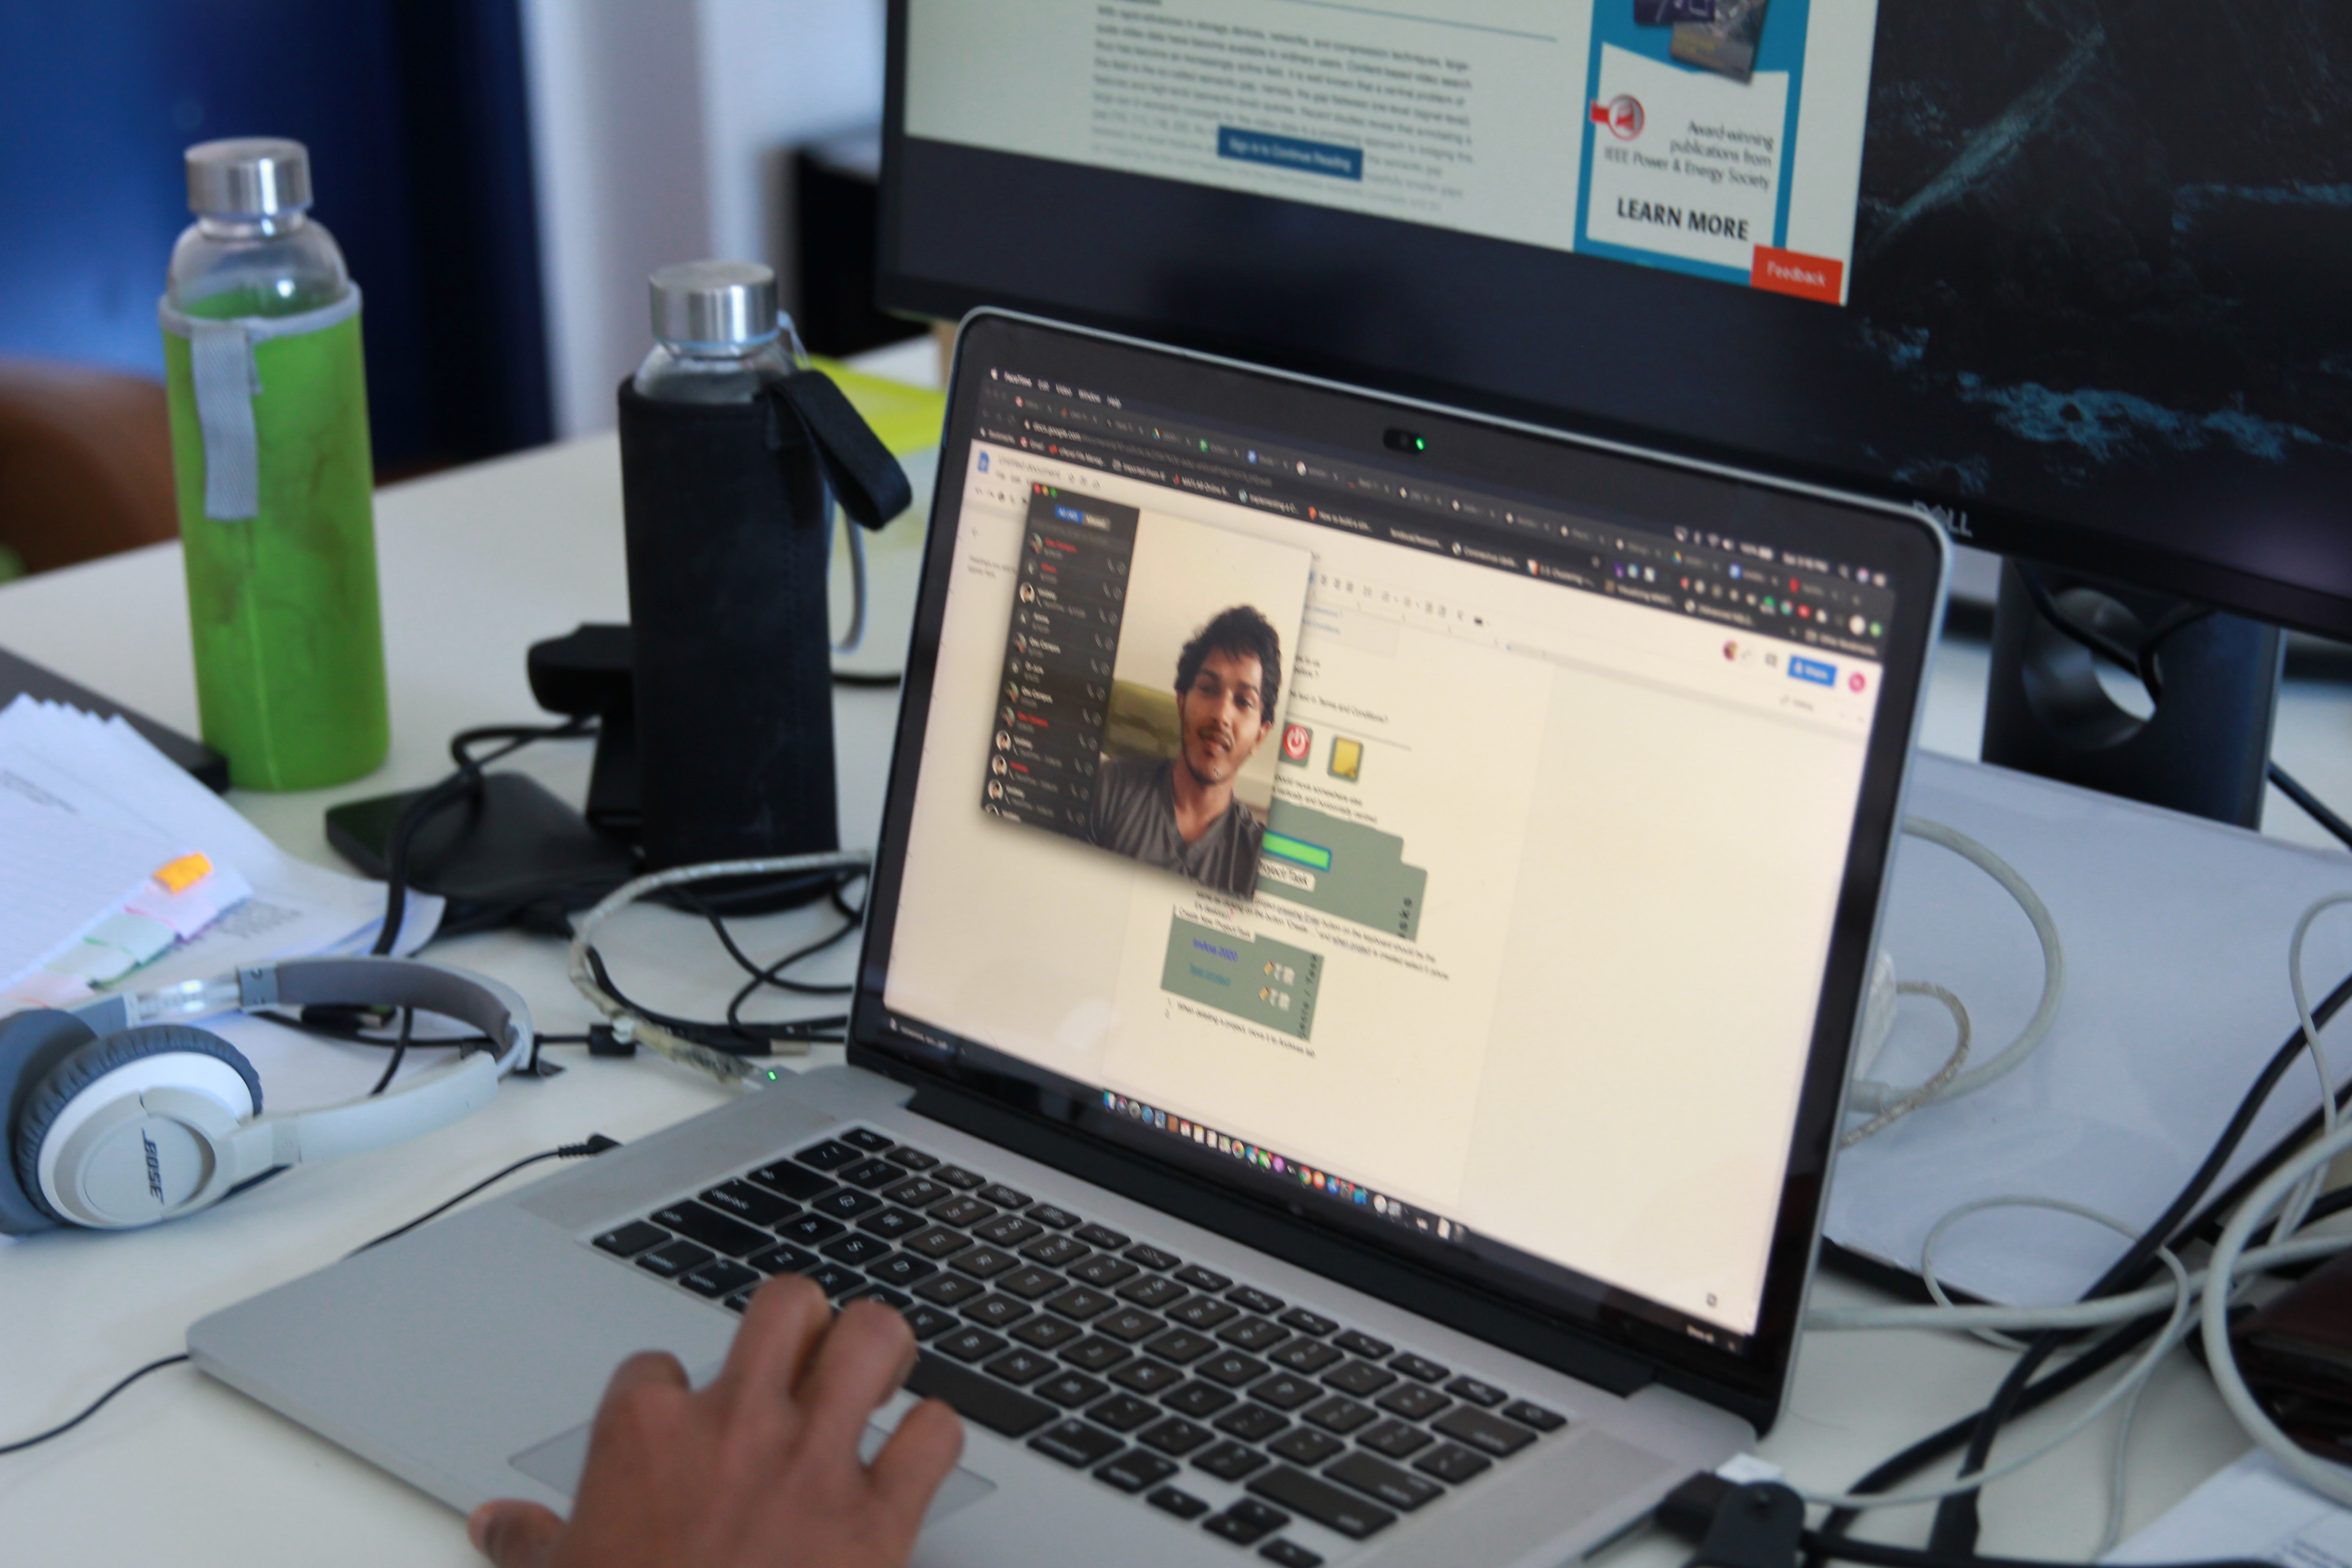
\includegraphics[width=\textwidth]{acmart-master-2/samples/nuwan.png}
  \caption{exciting concept art photo here. this is placeholder for now}
  \Description{photo of a user removing headphones.}
  \label{fig:teaser}
\end{teaserfigure}
%%
%% This command processes the author and affiliation and title
%% information and builds the first part of the formatted document.
\maketitle

\section{Introduction}
%Humans have been listening to music since 
% styles and types of music 
% instruments
% recent innovations in music, IR, AI 

\section{Background}
%paragraph 1: Humans instint of safety and the role of music 
%paragraph 2: trends of how music instruments have evolved

\section{Re-imagining the music interface}
% paragraph 1: music an experience that you can be immersed in without losing touch of reality

% music comes from emotions and we create music to retain, continue experiencing these emotions

\section{Design Scenarios}
% scenario : swimming in corals/alone in the forest. describe tech. add photos

% scenario: algorithms that easily convert our emotion stimuli into actual music

% discovering new music 
\section{Conclusion}

\section{Figures}

The ``\verb|figure|'' environment should be used for figures. One or
more images can be placed within a figure. If your figure contains
third-party material, you must clearly identify it as such, as shown
in the example below.
\begin{figure}[h]
  \centering
  \includegraphics[width=\linewidth]{sample-franklin}
  \caption{1907 Franklin Model D roadster. Photograph by Harris \&
    Ewing, Inc. [Public domain], via Wikimedia
    Commons. (\url{https://goo.gl/VLCRBB}).}
  \Description{The 1907 Franklin Model D roadster.}
\end{figure}

Your figures should contain a caption which describes the figure to
the reader. Figure captions go below the figure. Your figures should
{\bfseries also} include a description suitable for screen readers, to
assist the visually-challenged to better understand your work.

Figure captions are placed {\itshape below} the figure.

\subsection{The ``Teaser Figure''}

A ``teaser figure'' is an image, or set of images in one figure, that
are placed after all author and affiliation information, and before
the body of the article, spanning the page. If you wish to have such a
figure in your article, place the command immediately before the
\verb|\maketitle| command:
\begin{verbatim}
  \begin{teaserfigure}
    \includegraphics[width=\textwidth]{sampleteaser}
    \caption{figure caption}
    \Description{figure description}
  \end{teaserfigure}
\end{verbatim}

\section{Citations and Bibliographies}

The use of \BibTeX\ for the preparation and formatting of one's
references is strongly recommended. Authors' names should be complete
--- use full first names (``Donald E. Knuth'') not initials
(``D. E. Knuth'') --- and the salient identifying features of a
reference should be included: title, year, volume, number, pages,
article DOI, etc.

The bibliography is included in your source document with these two
commands, placed just before the \verb|\end{document}| command:
\begin{verbatim}
  \bibliographystyle{ACM-Reference-Format}
  \bibliography{bibfile}
\end{verbatim}
where ``\verb|bibfile|'' is the name, without the ``\verb|.bib|''
suffix, of the \BibTeX\ file.

Citations and references are numbered by default. A small number of
ACM publications have citations and references formatted in the
``author year'' style; for these exceptions, please include this
command in the {\bfseries preamble} (before
``\verb|\begin{document}|'') of your \LaTeX\ source:
\begin{verbatim}
  \citestyle{acmauthoryear}
\end{verbatim}


%%
%% The next two lines define the bibliography style to be used, and
%% the bibliography file.
\bibliographystyle{ACM-Reference-Format}
\bibliography{sample-base}
\nocite{*}

\end{document}
\endinput
%%
%% End of file `sample-acmtog.tex'.
